\documentclass[journal=jacsat,manuscript=suppinfo]{achemso}
%\usepackage{scicite}
\usepackage[sort&compress, numbers]{natbib}
\usepackage{times}
\usepackage{amssymb}
\usepackage{subfigure}
\usepackage{epsfig}
\usepackage{amsmath}
\usepackage{upgreek}
\usepackage{gensymb}
%\usepackage[colorlinks]{hyperref}
%\newcommand{\hah}[1]{\textcolor{magenta}{#1}}
\newcommand{\tws}[1]{\textcolor{red}{#1}}
\usepackage[version=4]{mhchem}
\usepackage{amsmath,amsfonts,amssymb,dcolumn,lscape,alltt,graphicx,chemarr}
\usepackage[english]{babel}
\SectionNumbersOn
\usepackage{bm}
\usepackage[T1]{fontenc}
\usepackage{chemstyle}
% NB added command for in line cite
\newcommand{\onlinecite}[1]{\hspace{-1 ex} \nocite{#1}\citenum{#1}}
% 2 column equations
%\usepackage{widetext, widetable}
%
\author{Benjamin~A.~Laws}
\email{b.laws@unsw.edu.au}
\affiliation{School of Chemistry, University of New South Wales, Sydney NSW 2052, Australia}
\alsoaffiliation{Research School of Physics, The Australian
	National University, Canberra ACT 2601, Australia}
\author{Zachariah~D.~Levey} 
\affiliation{School of Chemistry, University of New South Wales, Sydney NSW 2052, Australia}
\author{Andrei Sanov}
\affiliation{Department of Chemistry and Biochemistry, The University of Arizona, Tucson, Arizona 85721, United States}
\author{John F. Stanton}
\affiliation{Department of Chemistry, University of Florida, Gainesville, Florida 32611, United States}
\author{Timothy~W.~Schmidt} 
\affiliation{School of Chemistry, University of New South Wales, Sydney NSW 2052, Australia}
\author{Stephen~T.~Gibson}
\affiliation{Research School of Physics, The Australian
	National University, Canberra ACT 2601, Australia}
\title{Velocity Map Imaging Spectroscopy of C$_2$H$^-$ and C$_2$D$^-$: a benchmark study of vibronic coupling interactions}
\abbreviations{PES,PAD,EA,eKE,FWHM,VMI}
%\DeclareUnicodeCharacter{2192}{-}

\begin{document}

\tableofcontents
	

\section{C$_2$H$^-$ Spectral Assignments}
Spectral assignments for all peaks resolved in the photoelectron spectra of C$_2$H$^-$ from this work are presented in Table~\ref{tab:1}. Peaks are labelled with respect to the photoelectron spectrum of C$_2$H$^-$ at 300~nm in Figure~\ref{fig:1}. The experimental binding energy of each transition is given, alongside the anisotropy parameter sign ($+/-$), the corresponding vibronic symmetry, and the calculated energy from Ref.~\onlinecite{tar03}. Assignments are given as $\tilde{X}(v_1,v_2,v_3)\tilde{A}(v_1,v_2,v_3)$ where any superscripts represent hot-band transitions.

\begin{figure}[th!]
	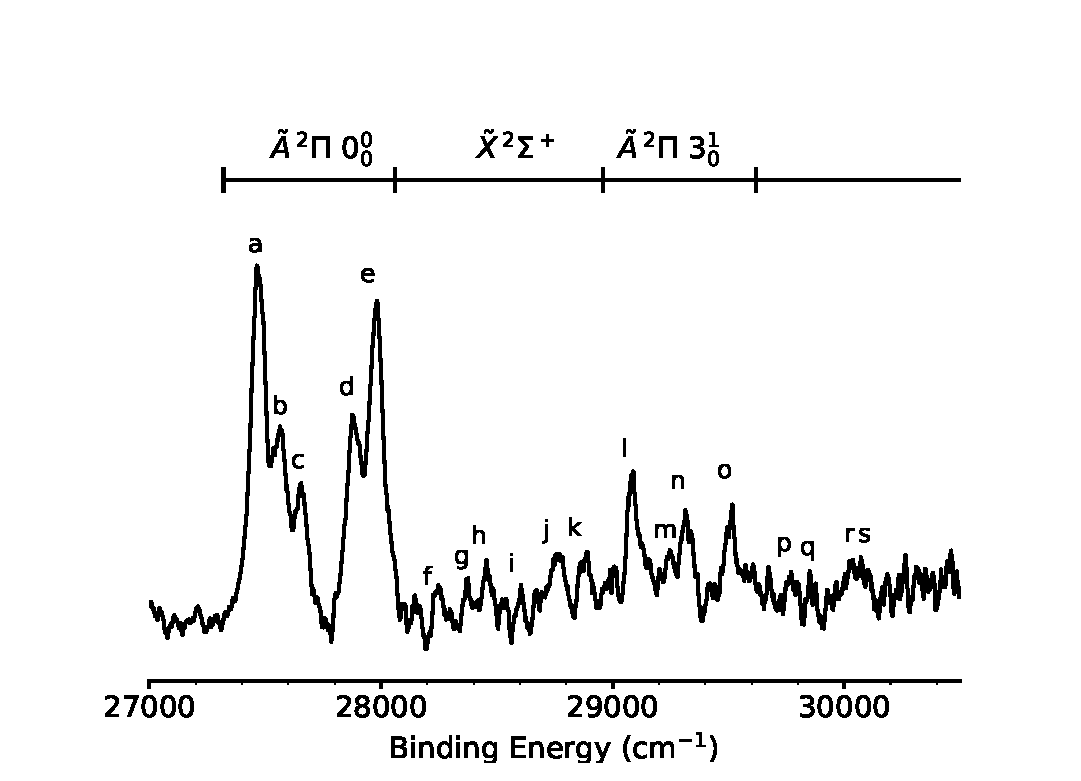
\includegraphics[width=0.6\textwidth]{figures/FigS1}
	\caption{Photoelectron spectrum of C$_2$H$^-$ at 300~nm, showing the alphabetic labelling of peaks used in this work.}
	\label{fig:1}
\end{figure}

\begin{table*}
	\caption{Peak positions (cm$^{-1}$), and assignments for the C$_2$H$^-$ photoelectron spectra from this work. The sign of the anisotropy parameter is shown for each transition, along with it's vibronic symmetry, and the calculated position from Ref.~\cite{tar03}.} \label{tab:1}
	\begin{tabular}{c c c c c c l}
		\hline Peak & eBE (cm$^{-1}$) & $v$ (cm$^{-1}$) & $\beta$ & Symmetry &  $v_{\text{calc}}\,^a$ & {Assignment}  \\ 
		 \hline \hline
		& 23 591 & -231 & + & $\Sigma^+$ & & $\tilde{X}(0,2^2,0)$ \\
		& 23 685 & -137 &  + & $\Sigma^+$ & & $\tilde{X}(0,1^1,0)$ \\
		& 23 823 & 0 & + & $\Sigma^+$ &  0 & $\tilde{X}(0,0,0)$ \\
		& 24 184 & 361 & $-$ & $\Pi$ & 371 & $\tilde{X}(0,1,0)$  \\
		& 24 630 & 807 & $+$ & $\Sigma^+$ & 794 & $\tilde{X}(0,2,0)$ \\
		& 25 663 & 1840 & $+$ & $\Sigma^+$ & 1838 & $\tilde{X}(0,0,1)$  \\
		& 25 916 & 2093 & $-$ & $\Pi$ & 2096 & $\tilde{X}(0,1,1)$  \\
		& 25 993 & 2170 & $-$ & $\Pi$ & 2166 & $\tilde{X}(0,5,0)$  \\
		& 26 362 & 2539 & $+$ & $\Sigma^+$ & 2536 & $\tilde{X}(0,2,1)$  \\
		& 26 757 &  2934 & $-$ & $\Pi$ & 2933 & $\tilde{X}(0,3,1)$  \\
		& 26 929 & 3106 & $-$ & $\Pi$ & 3104 & $\tilde{X}(0,7,0)$  \\
		& 27 175 & 3352 & + & $\Sigma^+$ & 3371 & $\tilde{X}(0,4,1)$ \\
		a & 27 430 & 3607 & $-$ & $\Pi$ & 3604 & $\tilde{X}(0,1,2)\tilde{X}(1,1,0)\tilde{A}(0,0,0)$  \\
		b & 27 515 & 3692 & $-$ & $\Pi$ & 3690 & $\tilde{X}(1,1,0)\tilde{X}(0,1,2)\tilde{A}(0,0,0)$   \\
		c & 27 612 & 3788 & $-$ & $\Pi$ & 3790 & $\tilde{X}(0,5,1)\tilde{A}(0,0,0)$  \\
		d & 27 851 & 4028 & $-$ & $\Pi$ & 4011 & $\tilde{X}(0,9,0)\tilde{X}(0,5,1)\tilde{A}(0,0,0)$  \\
		e & 27 941 & 4118 & $-$ & $\Pi$ & 4093 & $\tilde{X}(0,9,0)\tilde{A}(0,0,0)$  \\
		f & 28 200 & 4377 & $+$ & $\Sigma^+$ & 4375 & $\tilde{X}(0,6,1)$  \\
		g & 28 349 & 4526 & $+$ & $\Sigma^+$ & 4524 & $\tilde{X}(0,10,0)$  \\
		h  & 28 423 & 4600 & $-$ & $\Pi$ & 4593 & $\tilde{X}(0,3,2)\tilde{A}(0,0,0)$  \\
		i & 28 562 & 4739 & $-$ & $\Pi$ & 4702 & $\tilde{X}(0,7,1)\tilde{A}(0,1,0)$  \\
		j & 28 714 & 4891 & $-$ & $\Pi$ & 4879 & $\tilde{X}(0,7,1)$  \\
		k   & 28 834 & 5011 & $-$ & $\Pi$ & 5004 & $\tilde{X}(0,11,0)$  \\  
		l & 29 049 & 5226 & $-$ & $\Pi$ & 5222 & $\tilde{X}(0,1,3)\tilde{A}(0,0,1)$  \\
		m & 29 227 & 5404 & + & $\Sigma^+$ & 5406 & $\tilde{X}(0,12,0)\tilde{A}(0,1,0)$ \\
		n & 29 283 & 5460 & $-$ & $\Pi$ & 5445  & $\tilde{X}(0,5,2)\tilde{A}(0,0,1)$  \\
		o & 29 465 & 5642 & $-$ & $\Pi$ & 5630  & $\tilde{X}(0,9,1)\tilde{A}(0,0,1)$  \\
		p  & 29 740 & 5917 & $-$ & $\Pi$ & 5914 & $\tilde{X}(0,13,0)$ \\
		q & 29 844 & 6021 & + & $\Sigma^+$ & 6054 & $\tilde{X}(0,6,2)\tilde{X}(0,2,3)$ \\
		r & 30 021 & 6198 & $-$ & $\Pi$ & 6200 & $\tilde{X}(0,3,3)\tilde{A}(0,2,0)$ \\
		s & 30 086 & 6263 & $-$ & $\Pi$ & 6266 & $\tilde{X}(1,7,0)$ \\
	\end{tabular}
	\raggedright

$^a$ from calculations of Ref.~\onlinecite{tar03}
	
\end{table*}

\section{C$_2$D$^-$ Spectral Assignments}
Spectral assignments for all peaks resolved in C$_2$D$^-$ from this work are presented in Table~\ref{tab:2}. Peaks are labelled with respect to the photoelectron spectrum of C$_2$D$^-$ at 355~nm in Figure~\ref{fig:2}. The experimental binding energy of each transition is given, alongside the anisotropy parameter sign ($+/-$), the corresponding vibronic symmetry, and the calculated energy from Ref.~\onlinecite{tar03}. 

\begin{figure}[th!]
	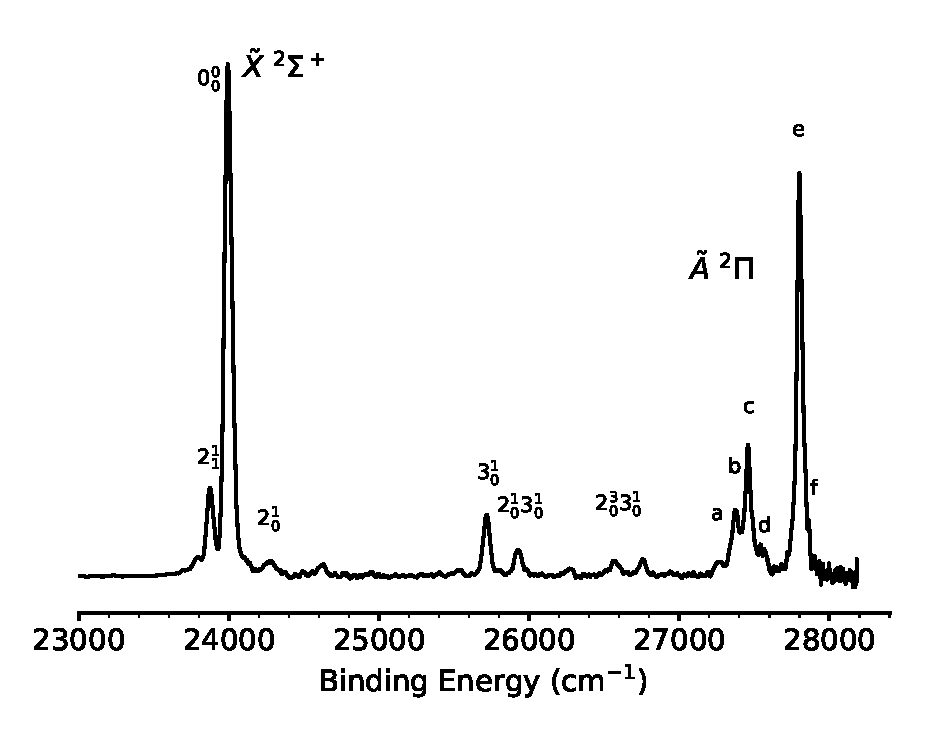
\includegraphics[width=0.6\textwidth]{figures/FigS2}
	\caption{Photoelectron spectrum of C$_2$D$^-$ at 266~nm, showing the alphabetic labelling of peaks used in this work.}
	\label{fig:2}
\end{figure}

\begin{table*}
	\caption{Peak positions (cm$^{-1}$) and assignments for the C$_2$D$^-$ photoelectron spectra from this work. The sign of the anisotropy parameter is shown for each transition, along with it's vibronic symmerty, and calculated position from Ref.~\cite{tar03}.} \label{tab:2}
	\begin{tabular}{c c c c c c c }
		\hline Peak & eBE (cm$^{-1}$) & $v$ (cm$^{-1}$) & $\beta$ & Symmetry &  $v_{\text{calc}}\,^a$ &{Assignment}  \\ 
		 \hline \hline
		& 23 751 & -197 & + & $\Sigma{+}$ & & $\tilde{X}(0,2^2,0)$ \\
		& 23829 & -120 & + & $\Sigma^+$ & & $\tilde{X}(0,2^1,0)$  \\
		& 23 949 & 0 & + & $\Sigma^+$ & 0 & $\tilde{X}(0,0,0)$ \\
		& 24 227 & 278 & $-$ & $\Pi$ & 287 & $\tilde{X}(0,1,0)$ \\
		& 24 577 & 629  & + & $\Sigma^+$ & 615 & $\tilde{X}(0,2,0)$ \\
		& 24 906 & 957 & $-$ & $\Pi$ & 953 & $\tilde{X}(0,3,0)$ \\ 
		& 25 506 & 1557 & + &  &  &  \\
		& 25 688 & 1740 & + & $\Sigma^+$ & 1744 & $\tilde{X}(0,0,1)$ \\
		& 25 901 & 1952 & $-$ & $\Pi$ & 1962 & $\tilde{X}(0,1,1)$ \\
		& 26 245 & 2297 & + & $\Sigma^+$ & 2302 & $\tilde{X}(0,2,1)$ \\
		& 26 556 & 2607 & $-$ & $\Pi$ & 2612 & $\tilde{X}(0,3,1)$ \\
		& 26 747 & 2798 & $-$ & $\Pi$ & 2796 & $\tilde{X}(1,1,0)$ \\
		a & 27 253 & 3304 & $-$ & $\Pi$ & 3309 & $\tilde{X}(0,5,1)$ \\
		b & 27 369 & 3420 & $-$ & $\Pi$ & 3426 & $\tilde{X}(1,3,0)$ \\
		c & 27 450 & 3501 & $-$ & $\Pi$ & 3511 & $\tilde{X}(0,1,2)$ \\
		d & 27 552 & 3603 & $-$ &  &  &  \\
		e & 27 793 & 3844 & $-$ & $\Pi$ & 3838 & $\tilde{A}(0,0,0)$\\
		f & 27 906 & 3957 & $+$ & $\Sigma^+$ & 3967 & $\tilde{X}(0,2,2)$ \\
	\end{tabular}
	
	\raggedright

	$^a$ from calculations of Ref.~\onlinecite{tar03}
\end{table*}



\newpage
\bibliography{sup-C2H}

\end{document} 